

\chapter{PHILLIPO}

PHILLIPO é um \emph{solver} para campos de deformação elástica em estruturas discretizadas por elementos finitos, e segue a simbologia e o padrão dos algoritmos descritos por Zienkiewicz em sua obra intitulada \emph{The Finite Element Method}, com algumas otimizações computacionais relacionadas a paralelismo e matrizes esparsas, e que visa constituir-se como referência didática na implementação legível e concisa dos algoritmos de elementos finitos em Julia no âmbito acadêmico do campus CCT, da UDESC. PHILLIPO é um programa de código aberto, que é distribuído em um repositório público\footnotemark[1]{} sob a licença LGPL\footnotemark[2]{}. Portanto, sua utilização é gratuita e livre para fins acadêmicos e comerciais, que incluem a modificação, implementação e venda de qualquer parte do programa, como também da documentação que o acompanha; só se resguarda, entretanto, a devida citação deste documento.
\footnotetext[1]{O repositório é mantido no GitHub, assim como o presente documento em formato Latex: \url{https://github.com/lucas-bublitz/PHILLIPO}}
\footnotetext[2]{O GiD, interface de pré e pós-processamento, é um software distribuído comercialmente, e não está sujeito à mesma licença que PHILLIPO.}

PHILLIPO foi idealizado, a princípio, como um projeto de aplicação do método de elementos finitos em um contexto de programação estruturada, porém, observou-se que essa abordagem é, senão obsoleta, já muito utilizada em pesquisas científicas. Portanto, optou-se em trazer uma visão de projeto de software, alterando o paradigma para a programação em despachos múltiplos (um forma alternativa à orientação a objetos), uma vez que tópicos envolvendo esses assuntos não são muito discutidos nas cadeiras dos cursos de engenharia (menos a de software, é claro), e que as vantagens desse tipo de abordagem vão desde a legibilidade do código, até o reaproveitamento de estruturas de dados e funções.

Um \emph{solver}, ou em melhor português, um solucionador em MEF não é uma novidade no mundo acadêmico, nem no comercial. Softwares como Calculix (que é distribuído integrado com o FreeCAD) e o FreeFEM, que já conta com 7 mil commits em seu repositório, são continuamente produzidos e aprimorados desde antes da virada do milênio, um trabalho que demanda tempo e uma comunidade bem ativa.

Destarte, a pretensão de PHILLIPO não é fornecer uma alternativa a esses softwares, muito menos servir de módulo ou biblioteca para agregar algum deles, além do mais, a elaboração de programas robustos e confiáveis é um trabalho demorado e de muitas pessoas. O próprio FreeFEM já conta com mais de 7 mil commits em seu repositório, com a participação de 41 desenvolvedores. 

A pretenção de PHILLIPO é construir uma aplicação simples utilizando o MEF, que possa aproveitar algumas ferramentas de contrução de código em Julia, como paralelismo e despachos múltiplos, para apresentar mais uma referência de programação em engenharia para os alunos do campus CCT, da UDESC, e, deste modo, evidenciar que é possível construir programas de engenharia de forma simples e legível, e que, por meio de uma linguagem de programação moderna, como Julia.

Neste capítulo é apresentado o funcionamento de PHILLIPO em duas partes. A primeira, descrevendo o flixo de execuçã normal do programa, isto é, utilizando o GID como interface de pré e pós-processamento, e, a segunda, esmiuçando o código, tanto do módulo PHILLIPO,  

\section{Fluxo de execução}

O fluxo de execução é uma ferramenta de projeto que tem como objetivo descrever a ordem e as condições que determinadas seções do código são executadas. A utilização de PHILLIPO.jl segue os digramas das figuras \ref{fig:fluxograma_GID} e \ref{fig:fluxograma_PHILLIPO}.
\begin{figure}
    \centering
    \caption{Fluxograma de execução: GID}
    \includegraphics[width = \textwidth]{Figuras/fluxograma_GID.pdf}
    \label{fig:fluxograma_GID}
\end{figure}

\begin{figure}
    \centering
    \caption{Fluxograma de execução: PHILLIPO.jl}
    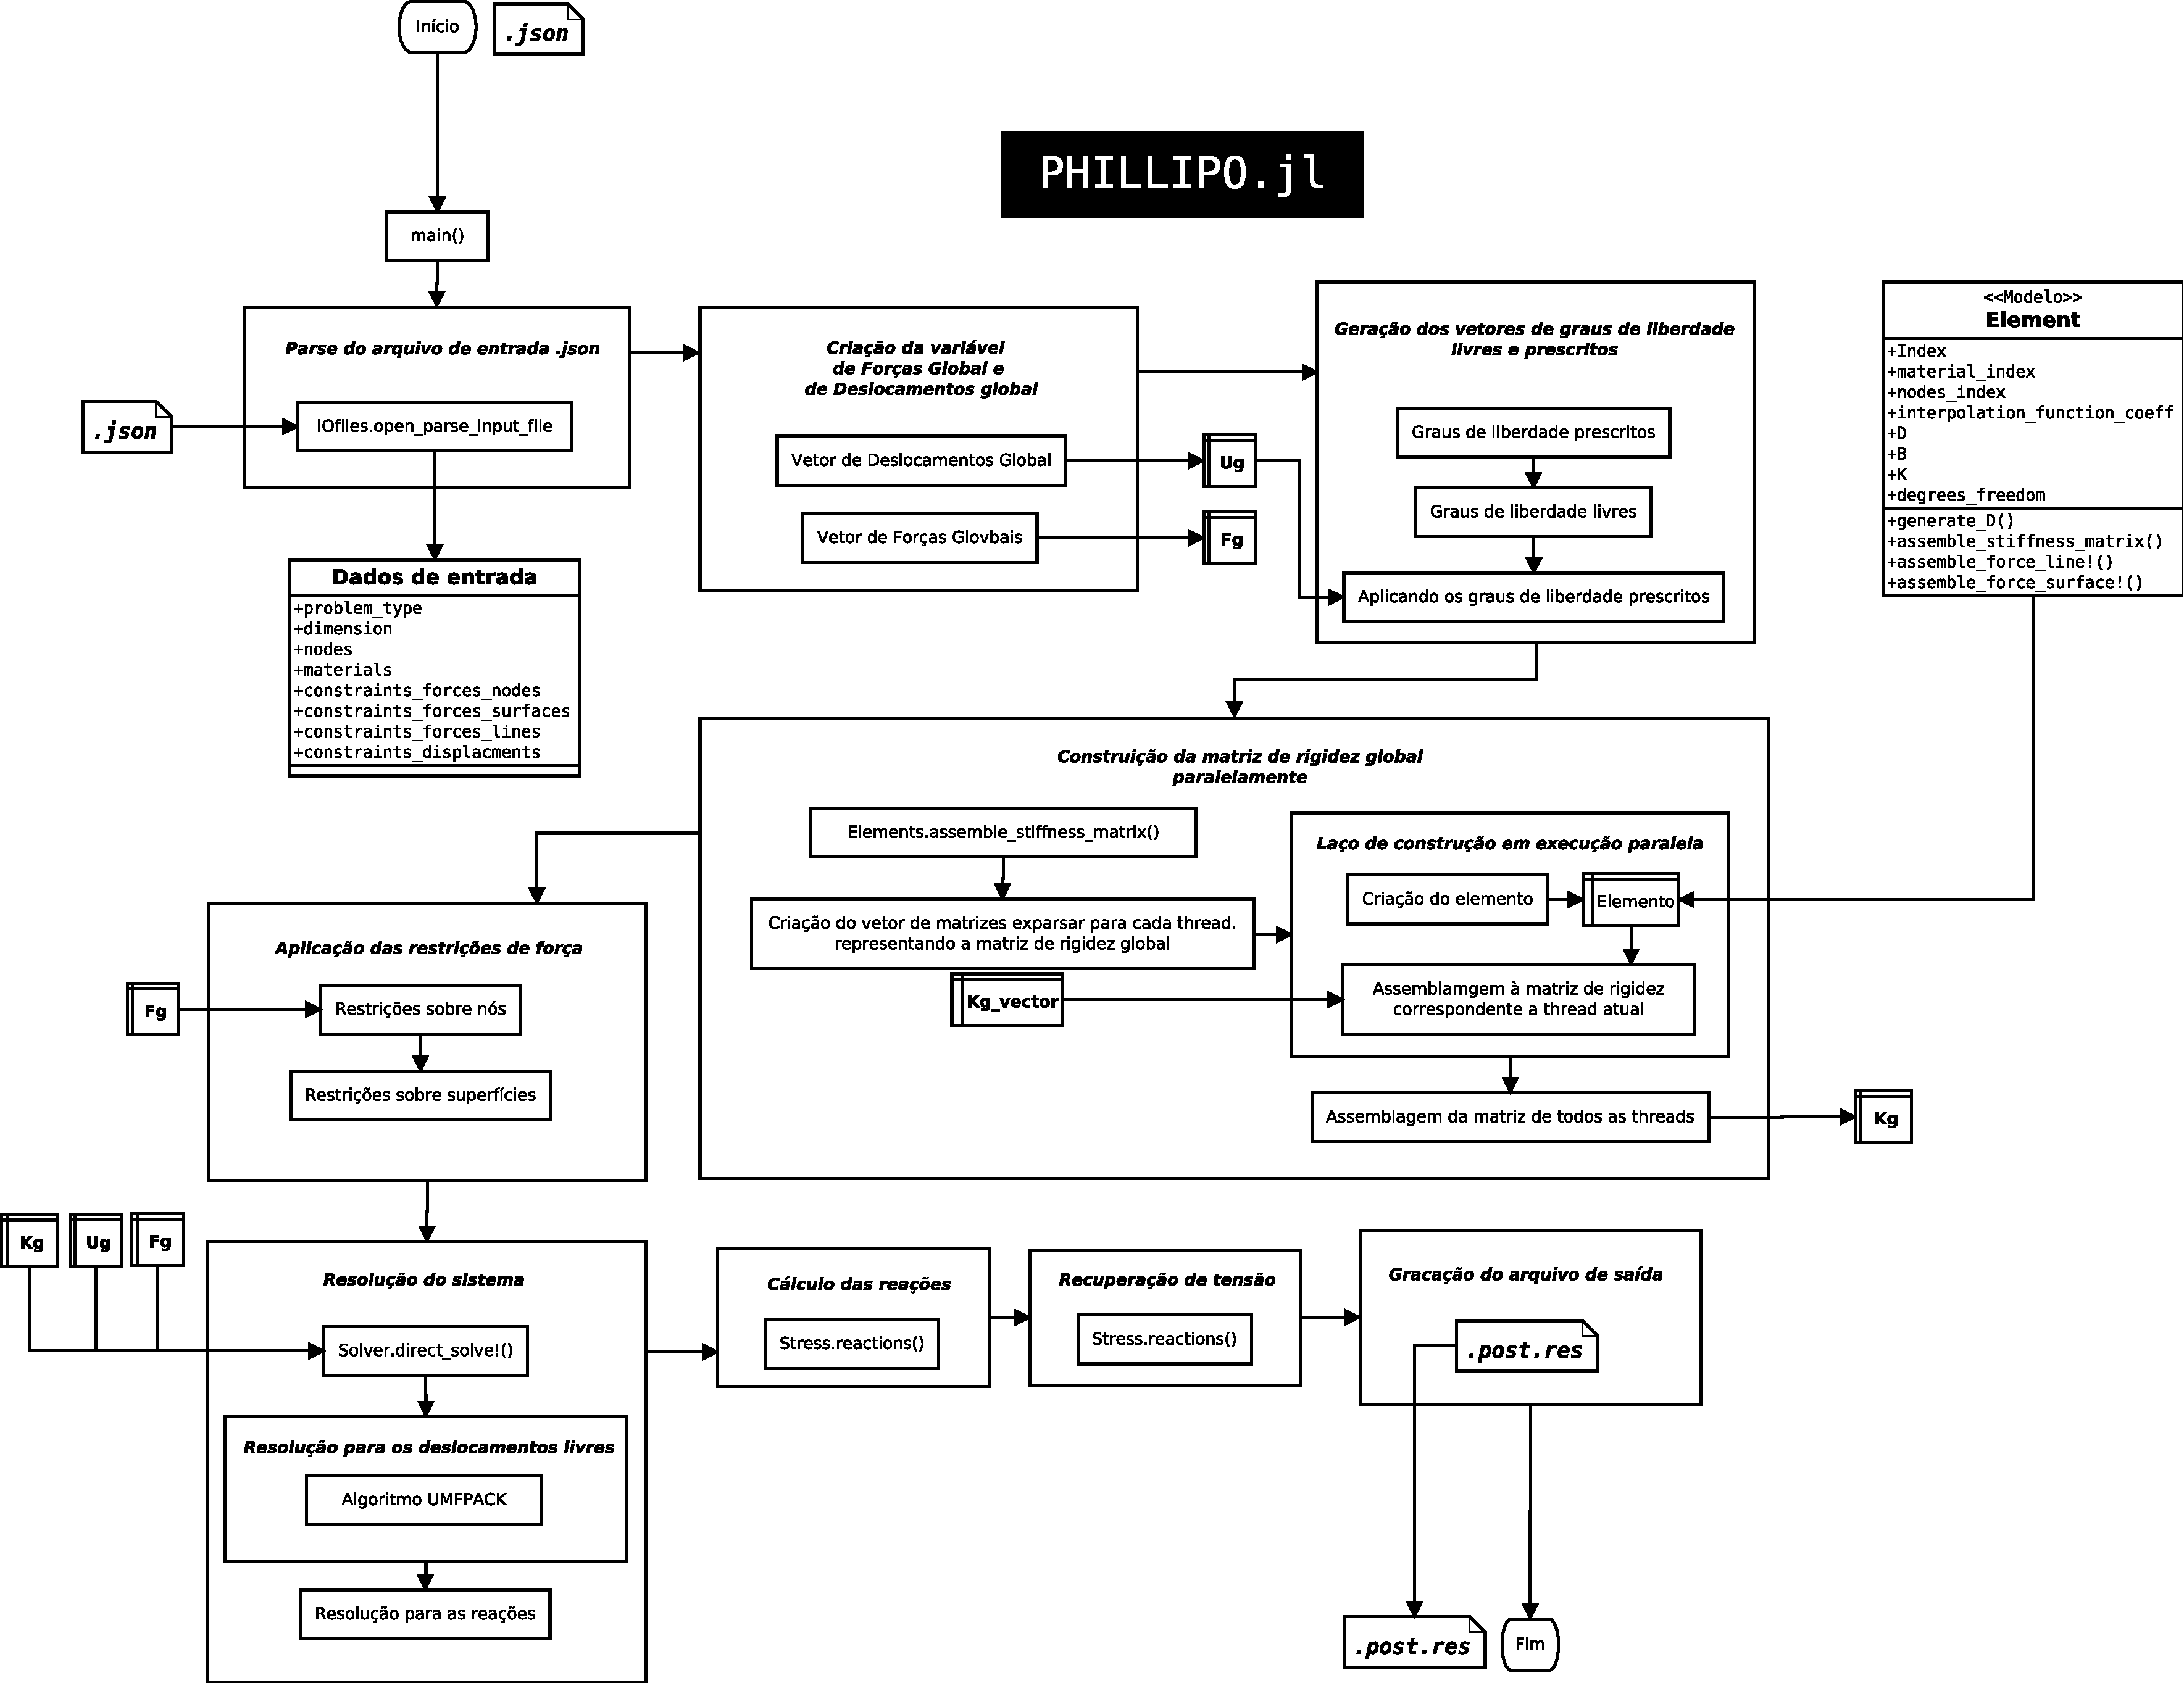
\includegraphics[width = \textwidth]{Figuras/fluxograma_PHILLIPO.pdf}
    \label{fig:fluxograma_PHILLIPO}
\end{figure}

Nesses diagramas, é possível separar a execução de uma utilização normal do software em três partes principais:

\begin{enumerate}
    \item Pré-processamento;
        Parte em que ocorre a criação da geometria, a definição das propriedades dos materiais, das condições de contorno e das cargas aplicadas, assim como a geração da malha e elementos.
    \item Processamento;
        Parte em que é chamada uma sessão Julia para carregar o módulo PHILLIPO.jl, que é responsável por ler os arquivos de entrada, e executar o algoritmo de elementos finitos, gerando os arquivos de saída para o GID.
    \item Pós-processamento;
        Parte em que o GID lê os arquivos de saída, e gera os gráficos de resultados.
\end{enumerate}

\section{GID}

O GID é um software utilizado como pré e pós-processamento, neste caso, para PHILLIPO. Nele é possível criar a geometria do problema, definir as propriedades dos materiais, as condições de contorno, as cargas aplicadas, e, principalmente, gerar a malha de elementos. Além de se ser possível sua integração com um \emph{solver} qualquer, por meio de um conjunto de arquivos de entrada e saída (ambos configurados de forma a permitir uma certa flexibilidade nessa integração), cuja execução é controlada por um \emph{script} em Batch, o que possibilita a automatização do processo de simulação. Nesta seção é abordado como é feita e integração entre o GID e PHILLIPO, por meio das pastas \emph{PHILLIPO.gid} e \emph{PHILLIPO3D.gid}, sendo que, como a nomeação dos arquivos sugere, a primeira é utilizada para problemas bidimensionais, e a segunda para problemas tridimensionais.

\subsection{PHILLIPO.gid}

O GID pode ser configurado para operar como pré e pós-processamentos de diversos programas, como o Abaqus, o Ansys, o Calculix..., por meio de um \emph{Problem type}, que é como o GID chama o conjunto de arquivos que configuram o formato de saída dos dados, a criação de determinadas propriedades para as condições de contorno e materiais, como também automatizar a execução da simulação, chamando o programa. Pode-se dizer que o \emph{Problem type} é uma interface para que as informações contidas no arquivo gerado pelo GID (geometria, malha, condições de contorno etc.) sejam salvas em um formato que o programa, o \emph{solver} no caso, possa interpretar, ao passo que o \emph{script} de execução automatiza o chamamento deste, e a simulação seja iniciada. 

Na pasta \emph{PHILLIPO.gid} é possível encontrar os seguinte arquivos:

\begin{enumerate}
    \item \emph{PHILLIPO.cnd}: define as condições de contorno e como são aplicadas;
    \item \emph{PHILLIPO.prb}: define as entradas de informações gerais;
    \item \emph{PHILLIPO.mat}: define as características dos materiais utilizados para os elementos;
    \item \emph{PHILLIPO.bas}: configura o arquivo de saída do GID para ser interpretado por PHILLIPO.jl;
    \item \emph{PHILLIPO.bat}: \emph{script} para chamar uma sessão Julia, chamando \emph{link.jl};
    \item \emph{link.jl}: importa o módulo PHILLIPO e o executa.
\end{enumerate}

O primeiro arquivo do \emph{Problem type} de PHILLIPO é \emph{PHILLIPO.cnd}, que define as condições de contorno e sobre quais entidades, leia-se nós, elementos ou geometrias (superfícies, volumes, linhas etc.), são aplicadas, por meio de uma sintaxe específica \footnote{No manual do usuário do GID, acessível em \url{https://gidsimulation.atlassian.net/wiki/spaces/GUM/overview}, é possível encontrar a descrição o funcionamento de toda essa sintaxe, que compreende desde esse arquivo de condições de contorno, como também, dos outros que compões a construção do \emph{problem type}.}, uma forma de marcação de texto, que é interpretada pelo GID.

\begin{figure}
    \lstinputlisting[language=json, lastline=10]{../GID connection/PHILLIPO.gid/PHILLIPO.cnd}
    \caption{Parte do arquivo de condições de contorno: PHILLIPO.cnd}
    \label{fig:PHILLIPO.cnd}
\end{figure}

Em sua representação parcial, da figura \ref{fig:PHILLIPO.cnd}, é possível notar a construção de uma condição de contorno por meio de um bloco que inicia na linha 1, com a expressão \emph{CONDITION: Constraint_\underline{}displacement\underline{}point}, que também nomeia esta condição, referente a restrição de deslocamento em pontos (entidade geométrica discretizada por um nó), e que acaba com \emph{END CONDITION}. Dentre essas linhas, são definidas as formas e os valores que essa condição vai aplicar sobre a geometria selecionada, neste caso, os pontos. Na linha 2, é definido, justamente, sobre qual entidade geométrica se aplica essa condição: pontos. Na próxima linha, é definido como que essa informação, que foi associada à entidade geométrica se traduz na malha, neste caso, essa condição é aplicada sobre os nós que correspondem aos pontos, ou seja, quando o GID for gerar a malha, vai aplicar essa condição para o nó que corresponde ao ponto.\footnote{Isso se deve porque a malha é criada sobre a geometria, posteriormente à aplicação das condições de contorno sobre aquela.}

As linhas seguintes, 4 a 9, se referem aos valores da condição, neste caso, aos deslocamentos dos nós nas direções de \emph{X}, \emph{Y} e \emph{Z}, e seus valores padrão, nesse caso, 
